\subsection{Verbesserung der UI und der Bedienbarkeit}

Neben der Funktionalität, spielen das Aussehen und die Bedienbarkeit einer Software eine große Rolle. Eine Software sollte möglich intuitiv bedienbar sein und dem Benutzer bei der Bedienung durch Hinweise und Erklärungen Hilfestellung leisten können. 

\subsubsection{Kosmetische Änderungen}
Ob eine Software mit Hilfe von Java Swing erstellt wurde, kann häufig am Aussehen festgestellt werden. Das liegt am von Swing als Standard eingestellten \emph{\acrfull{lnf}}, dem sog. \glqq Metal\grqq{}-Theme. Das \acrshort{lnf} verändert, wie der Name schon sagt, das Aussehen und Verhalten von Swing-Komponenten. Der Vorteil des Metal-\acrshort{lnf}s ist, dass es cross-platform ist und daher unabhängig vom zugrundeliegenden Betriebssystem eingesetzt werden kann. Der Nachteil ist das teils veraltete Aussehen und die stellenweise schwierige Bedienung. Als Beispiel ist in Abb. \ref{fig:metalFileSelection} eine Dateiauswahl mit dem Metal-\acrshort{lnf} dargestellt. 

\begin{figure}
    \centering
    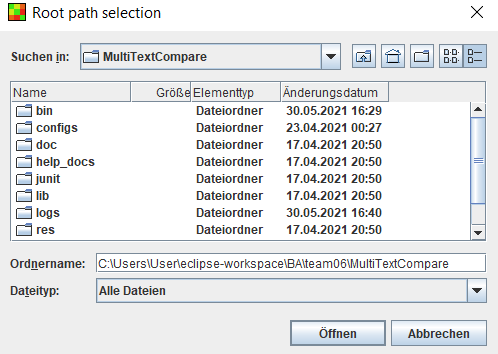
\includegraphics[]{images/metalFileSelection.png}
    \caption{Dateiauswahl unter Metal-\acrshort{lnf}}
    \label{fig:metalFileSelection}
\end{figure}

Als Alternative existieren unter Swing noch weitere, vom Betriebssystem abhängige \acrshort{lnf}s. Diese können mit der Zeile
\begin{minted}{java}
UIManager.setLookAndFeel(UIManager.getSystemLookAndFeelClassName());
\end{minted}
automatisch beim Programmstart geladen und angewandt werden. Zwar ist MultiTextCompare zunächst nur als Windows-Software geplant, allerdings wurde sie bisher immer so entwickelt, dass sie auch auf anderen Betriebssystemen lauffähig ist. Deswegen wird immer das dem Betriebssystem zugehörige \acrshort{lnf} geladen. Die in Abb. \ref{fig:windowsFileSelection} gezeigte Dateiauswahl wirkt dank dem Windows-\acrshort{lnf} nun verständlicher und etwas moderner. Unter Linux würde, sofern es installiert ist, bspw. dann das GTK+ \acrshort{lnf} geladen werden \autocite{lookAndFeel}.

\begin{figure}[!htb]
    \centering
    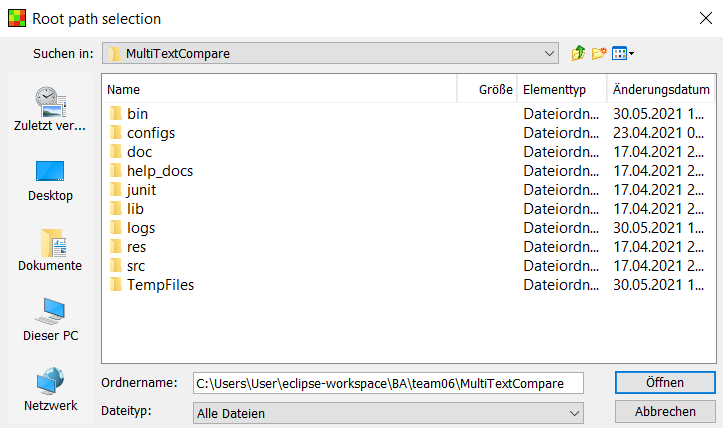
\includegraphics[scale=0.8]{images/windowsFileSelection.png}
    \caption{Dateiauswahl unter Windows-\acrshort{lnf}}
    \label{fig:windowsFileSelection}
\end{figure}

\newpage\subsubsection{Bedienung der Ähnlichkeitsmatrix}

Eine der Anforderungen ist, dass die Software einfach zu bedienen sein soll, jedoch ist die Auswahl der Dateien zur Anzeige der Diff in Version 1.0 in dieser Hinsicht noch nicht optimal. Ein Klick auf eine Zelle innerhalb der Ähnlichkeitsmatrix öffnete eine Diff-Anzeige für die beiden Dateien in der jeweiligen Zeile bzw. Spalte. Um drei Dateien auszuwählen, musste der Benutzer die Spaltenköpfe der Matrix anklicken, was mehrere Probleme beinhaltet. Zum einen musste für jede Datei einzeln die Ähnlichkeit zu anderen Dateien nachgeschaut werden, da die Matrix nicht automatisch die zugehörigen Zellen der ausgewählen Spaltenköpfe gesondert anzeigt. Zum anderen war es nicht möglich nach dem Fund zweier ähnlicher Dateien nach einer dritten ähnlichen Datei zu suchen ohne die ersten beiden immer wieder auszuwählen. Aus diesen Gründen soll das Auswahlsystem komplett überarbeitet werden.

Zunächst sei grundlegend zu erwähnen, dass die Ähnlichkeitsmatrix technisch gesehen eigentlich keine Matrix ist, da diese nicht als Swing-Komponenten existieren. Stattdessen wird eine JTable verwendet, die als erste Spalte Zellen besitzt, die das Aussehen und Verhalten der Spaltenköpfe aus der JTable imitieren. Dies wird durch eine angepasste Version der Klasse \emph{RowNumberTable} von Rob Carrick umgesetzt \autocite{rowNumTable}. Jegliche Funktionen um Klicks des Benutzers innerhalb der Matrix zu bearbeiten basieren also auf den vorgegebenen Funktionen der Klasse JTable. Das Event-Handling dieser Klicks passiert in einer zusätzlichen Handler-Klasse namens \emph{MouseAdapterMatrix}. Diese erbt von der Swing-nativen Klasse \emph{MouseAdapter} und implementiert die Handler-Methode \emph{mousePressed}(), welche das zu handlende Event als Übergabeparameter erhält. 

Praktischerweise lassen sich aus diesem Event die Zeile und Spalte des Klicks auslesen. Da die RowNumberTable die JTable der Matrix einschließt und kein tatsächlicher Teil der klickbaren Matrix ist, verändern sich auch die Indices nicht. 

Um eine Diff-Anzeige zu öffnen soll nun ein Doppelklick notwendig sein, da ein einzelner Klick einfacher zu Fehlklicks führen kann und diese je nach Dateigröße auch eine Wartezeit nach sich ziehen können. Um einen Doppelklick zu erkennen lässt sich die Methode \emph{getClickCount}() auf dem Eventobjekt ausführen. Um drei Dateien auszuwählen, soll nun ein Zwischenschritt eingeführt werden. Zunächst soll es möglich sein eine Zelle als Referenz festzulegen. Dabei werden alle Zellen, die nicht innerhalb der gleichen Zeile und Spalte oder auf der Hauptdiagonale liegen, ausgegraut und sollen damit nicht klickbar sein. Dies führt dazu, dass jeder mögliche Vergleich übersichtlich dargestellt wird und immer genau drei Dateien ausgewählt werden können. Diese Auswahl geschieht dann mit einem weiteren Klick auf eine der farbigen Zelle und führt nicht dazu, dass die Referenzzelle zurückgesetzt wird. Dafür muss der Renderer der JTable wissen, welche Zelle gerade die Referenzzelle ist.

Für solche Fälle existiert eine zentrale Klasse \emph{Management}, die nach dem Singleton-Entwurfsmuster Objekte für sämtliche Klassen instanziiert, von denen genau eine Instanz existieren soll. Zudem können dort Variablen gespeicht werden, die an verschiedenen Stellen im Code gebraucht werden und ebenfalls nur einmal existieren sollten. Beispiele dafür sind die aktuelle Konfiguration der Software oder die eben erwähnte aktuelle Referenzzelle. Für den sog. \emph{TableCellRenderer} wurde die \emph{prepareRenderer}()-Methode so überschrieben, dass sie prüft ob ein boolsches Flag durch die MouseAdapterMatrix im Management gesetzt wurde und dann entweder die Matrix komplett oder nur die Zellen nach den o.\,g. Kriterien koloriert. Das Resultat ist in Abb. \ref{fig:matrixGrau} zu sehen.

\begin{figure}
    \centering
    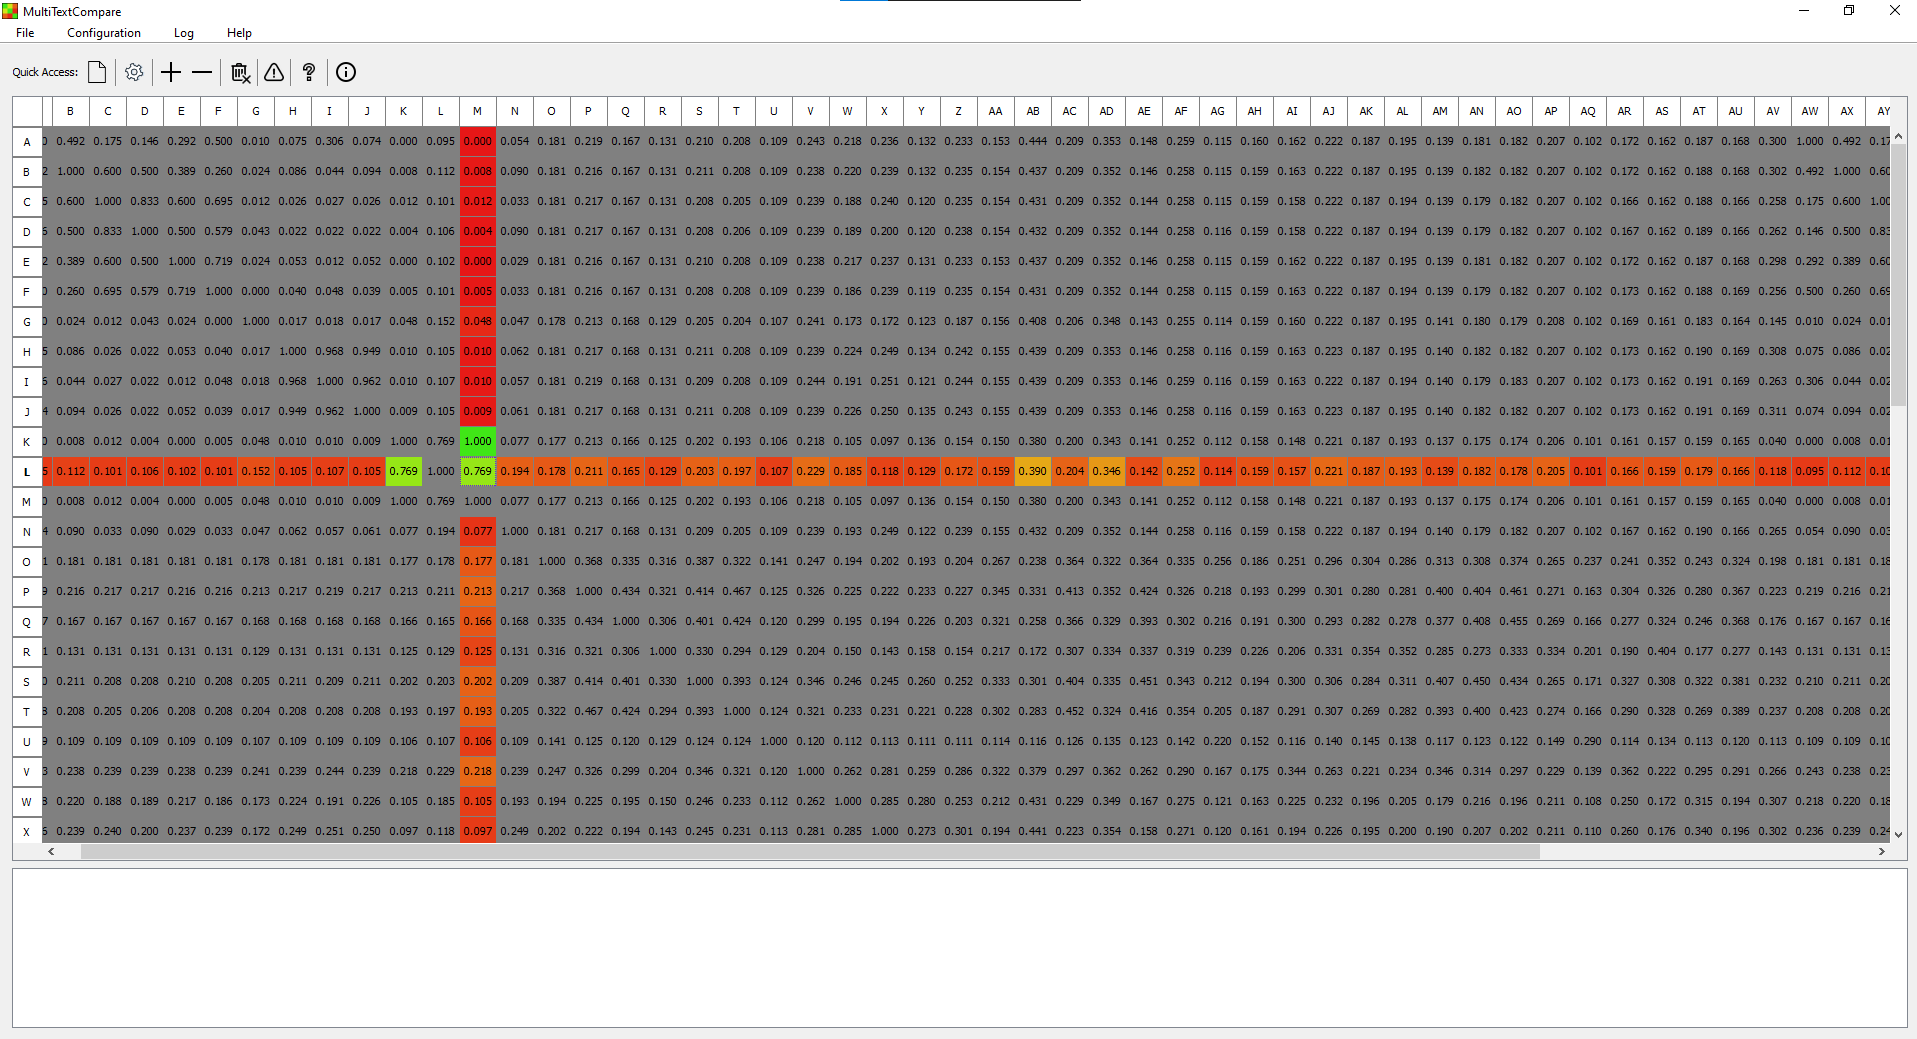
\includegraphics[width=\textwidth]{images/Matrix_neu.png}
    \caption{Ausgrauen der Matrix}
    \label{fig:matrixGrau}
\end{figure}


\subsubsection{Konfiguration}

Im Laufe dieser Arbeit wurden bereits diverse konfigurierbare Parameter besprochen. Darunter fällt u.\,a. die Auswahl der Vergleichsmodi, die Funktionsweise des Matchings, Parameter zum Sortieren oder Normieren der Inputdateien. Zwar erhöht eine größere Anzahl an Konfigurationsparametern die Komplexität der Software für Benutzer und Entwickler, zeitgleich liefert sie aber auch die Möglichkeit die allgemeinen Funktion des Textvergleichs für die zu vergleichenden Dateien anzupassen. Schließlich sind die vorgestellten Vergleichsalgorithmen lediglich Approximationen der Ähnlichkeit von Dateien nach bestimmten Kritierien und bilden daher keine objektive Bewertung für alle möglichen Arten von Wissensrepräsentation innerhalb der unterstützten Dateiformate. Falls der Benutzer Dateien vergleichen möchte, die nicht ideal mit den aktuellen Parametern verglichen werden würden, wäre es sinnvoll mehrere Konfigurationsdateien erstellen zu können und diese einfach auszutauschen anstatt immer wieder die aktuelle Konfiguration zurückzusetzen oder zu überschreiben.

MutliTextCompare erstellt, falls noch nicht vorhanden, eine Standardkonfiguration basierend auf Key-Value Paaren für jeden Parameter. Um eine alternative Konfiguration zu verwenden, wird in der Standardkonfiguration ein weiteres Feld für den Pfad der aktuellen Konfigurationsdatei hinterlegt. Ist dieses nicht leer und die Datei existiert, wird diese Konfiguration verwendet, ansonsten wird die Standardkonfiguration verwendet. Der Benutzer hat dadurch die Möglichkeit die aktuelle Konfiguration über die UI zu überschreiben oder als neue Datei unter Angabe des Dateinamens zu erstellen.

\subsubsection{Persistenz von Vergleichen}

Trotz der bisher durchgeführten Optimierungen für die Vergleiche und das Matching, können Vergleiche mit vielen, großen Dateien durchaus noch einige Minuten dauern. Solche langen Wartezeiten können sehr unangenehm sein, besonders wenn die gleichen Vergleichsergebnisse zu einem späteren Zeitpunkt wieder gebraucht werden. Es ist allerdings in Java bspw. durch Serialisierung möglich, bestimmte Programmteile persistent zu speichern. 

Nach Erstellung und Anzeige der Ähnlichkeitsmatrix wird die Diff für Dateien erst berechnet, wenn sie vom Benutzer ausgewählt wurden. Falls vergleichsbezogene Parameter geändert werden, muss die Matrix neu berechnet werden, um diese zu sehen. Das heißt, dass es ausreicht genau den Programmzustand wiederherzustellen, bei dem die Matrix gerade erzeugt wurde. Innerhalb des Codes wird dafür die Liste mit den berechneten Vergleichen der Matrix benötigt. Zusätzlich muss die Map der \emph{FileImporter}-Komponente gespeichert werden, die die erstellten temporären Dateien auf die Originaldateien mappt. Letztlich wird eine geordnete Liste der ausgewählten Dateien  bzw. ihrer Dateipfade mit zugehörigem Index gespeichtert. Zwar könnte diese Liste aus der Map wiederhergestellt werden, allerdings müssten dafür einige Methoden zentralisiert oder publik gemacht werden, was die Abhängigkeiten der Klassen und damit die Komplexität der Code-Base weiter erhöht.

Für die persistente Speicherung über Serialisierung muss sichergestellt werden, dass alle zu speichernden Objekte das Interface \emph{Serializable} implementieren. Dies muss nur für die selbst erstellte Matrix bzw. die Klasse \emph{ICompareImpl} nachgeholt werden. Um die Objekte zu serialisieren wird die native Java Klasse \emph{ObjectOutputStream} verwendet und mit einem \emph{FileOutputStream} in eine Datei geschrieben. Der Dateiname ist vom Benutzer wählbar und besitzt immer die Dateiendung \emph{.mtc}. Damit die Objekte korrekt ein- und ausgelesen werden können, müssen diese in der gleichen Reihenfolge geschrieben und gelesen werden.

Da die Map des FileImporters nur Referenzen auf die Dateien enthält, muss noch sichergestellt werden dass die temporären Dateien eines Vergleichs mitgespeichert werden um die an den Dateien vorgenommenen Normierungen und Sortierungen korrekt anzuzeigen. Dafür wird für jeden gespeicherten Vergleich ein Verzeichnis erstellt, indem sowohl die mtc-Datei mit den gespeicherten Objekten, als auch ein Verzeichnis mit den zugehörigen temporären Dateien vorliegt. Diese temporären Dateien werden dann in das \emph{TempFiles}-Verzeichnis der Software kopiert sobald der jeweilige Vergleich geladen wurde.

\subsubsection{Benutzerfeedback und Logging}\label{logging}

Beim Öffnen von MultiTextCompare erscheint in der unteren Hälfte des Panels ein Log. Dieser dient dazu, dem Benutzer Feedback zu seinen Aktionen zu liefern, bspw. wenn eine Referenzzelle bei der Auswahl von Dateien für die Diff-Anzeige selektiert wird. Zusätzlich werden so Fehler beim Parsen oder interne Fehler während der Laufzeit an den Benutzer weitergegeben. Bisher gab es jedoch keine Unterscheidung nach der Schwere des Fehlers oder der Wichtigkeit der Nachricht, was durch eine interne Logging-Komponente geändert werden soll. Wie bereits im Kapitel zu Architektur in \ref{architektur} gezeigt wurde, funktioniert diese Logging-Komponente außerhalb der eigentlichen 3-Schichten-Architektur. 

Es existiert zwar im Paket \emph{java.util.logging} bereits eine native Logging-Lösung, aber sie ist hier fast schon zu umfangreich und benötige mehr Arbeit um sie in die Code-Base einzupflegen. In der eigenen Logger-Komponenete werden nur 3 Log-Level unterschieden: 
\begin{description}
\item[Info] Beinhaltet das Feedback zur User-Interaktion und Benachrichtigungen über Berechnungen wie den Beginn des Vergleichs und das Ende mit der Berechnungsdauer. Hier handelt es sich um optionale Ausgaben, die besonders dann signifikant sind, wenn eine Berechnung länger dauert oder sich der Benutzer bei der Bedienung der Software noch nicht sicher ist. Diese Ausgaben werden als regulärer Text im Log hinterlegt.

\item[Warning] Bei diesem Level werden Fehler aufgeführt die entweder durch falsche Benutzung der Software auftreten oder durch fehlerhafte Inputdateien. Ein Beispiel für falsche Benutzung wäre z.\,B. der Versuch einen Vergleich persistent zu speichern bevor überhaupt eine Matrix erzeugt wurde. Warnings führen nicht zu Fehlverhalten und werden mit roter Schrift auf gelbem Hintergrund im Log angezeigt.

\item[Error] Errors sind schwerwiegende Fehler, die dazu führen dass das Programm nicht ordnungsgemäß funktionieren kann. Der wahrscheinlichste Fehler auf diesem Level ist eine \emph{FileNotFoundException}, die geworfen wird falls Dateien unerwartet gelöscht, verschoben oder umbenannt wurden. Diese Fehler werden im Log mit rotem Hintergrund und weißer Schrift angezeigt.
\end{description}

Zusätzlich zur Anzeige im Log werden diese Ausgaben auch persistent in Logdateien gespeichert. Um riesige Logdateien und damit einen Verlust der Übersicht zu vermeiden, werden die Logs nach Datum getrennt. Für jede Logausgabe wird dafür geprüft ob eine aktuelle Logdatei existiert, ansonsten wird eine neue Datei erstellt. Zwar werden alle Logausgaben unabhängig vom Level in die Logdateien geschrieben, dem Benutzer ist es aber möglich einzelne Level für die Anzeige im Log ein- und auszuschalten.
